
\chapter{First Experimental Evaluation Cycle}

    \xexeo{Todo capítulo deve ter uma introdução explanatória. "This chapter describes"}
    \vitor{Feito.}

    % This chapter describes the first experimental cycle of this research, structured according to the DSR methodology, as detailed in Section~\ref{sec:dsr-application}. It situates the experiment within the established \textbf{context} of knowledge management in the well construction and maintenance domain of a major oil company. The core \textbf{problem} this experiment addresses is the need for an effective mechanism to query complex technical and operational information within large volumes of unstructured data. As a solution, this experiment proposes and implements two distinct \textbf{artifacts}: a single-agent system and a multi-agent architecture, both designed to leverage LLMs for responding to specialized user queries. Finally, the chapter details the \textbf{evaluation} of these artifacts, outlining the methodology, the dataset creation process, and the metrics (Truthfulness, Performance, and LLM Cost) used to assess their capabilities and limitations.

    \xexeo{Acho que pode até ser Primeiro Ciclo, ou pode ter um nome como ``Efetividada das LLMs na Solução..''  vai ter que quebrar esse capítulo, que tem muita informação nos conceitos da DSR: no mínimo nos quatro principais: Contexto, Problema, Artefato, Avaliação. Grande parte do contexto e problema já devem ser descritos no capitulo que eu pedi para criar e aqui só faz referência.}
    \vitor{O Capítulo foi refatorado para ficar alinhado com a DSR.}

    \xexeo{Ok, você foi direto para o experimento mas não disse o que ia fazer. Aqui exatamente cabe o quadro da DSR que eu te mandei: qual o contexto, qual o problema, qual a suposição (de utilidade ou de mundança de contexto), qual os quadro teóricos, qual o(s) artefato(s) proposto(s) e como serão avaliados, vai fechar muito bem.}
    \vitor{O Capítulo foi refatorado para ficar alinhado com a DSR.}

    
    \xexeo{isso aqui é a validação, mas qual é o problema, qual a proposta, são essas informações que faltam para ficar bem organizado} 
    \vitor{O Capítulo foi refatorado para ficar alinhado com a DSR.}

    This chapter describes the first experimental cycle of this research, as introduced in Section~\ref{sec:dsr-application}, conducted to investigate the effectiveness of different LLM based agent architectures. The primary objective is to address complex, domain-specific queries within the field of well construction and maintenance. This initial cycle serves as a foundational study, comparing single-agent and multi-agent systems to generate empirical insights into their performance, cost, and inherent limitations. The findings from this cycle will inform the more advanced, quantitative evaluation performed in the second experiment.

    Following the principles of DSR, this chapter is structured to clearly present the research components. We will begin by defining the business context and the specific problem this experiment aims to solve. Subsequently, we will describe the design of the proposed technological solutions, referred to as artifacts. Finally, we will detail the evaluation methodology, including the process for data set creation, the metrics used for assessment, and a thorough analysis of the results.
    
    \section{Design Science Research Framework}
    
        To provide a clear and organized structure for this experiment, we adopt the DSR framework. The key components of this research cycle are outlined as follows:

        \begin{description}
            \item[Context] The operational environment of the well construction department within a major oil company, where efficient access to technical knowledge is critical.

            \item[Problem] The challenge faced by engineers and specialists in effectively querying and retrieving accurate information from vast, unstructured, and domain-specific knowledge bases (e.g., operational reports, lessons learned).

            \item[Supposition] Our core supposition is that LLM-based agent systems can improve the efficiency and accuracy of information retrieval for specialized tasks, but that the choice of architecture (single-agent vs. multi-agent) will have a measurable impact on performance and cost.

            \item[Theoretical Frameworks] This work is grounded in the theories of Intelligent Agents, Retrieval-Augmented Generation (RAG), and multi-agent systems, as detailed in the Literature Review.

            \item[Proposed Artifacts] Two distinct LLM-based agent systems are proposed and built:
            \begin{itemize}
                \item A Single-Agent Architecture.
                \item A Multi-Agent Architecture.
            \end{itemize}

            \item[Evaluation] The artifacts are evaluated by a panel of domain experts who assess the quality of their responses to a curated set of real-world queries. The evaluation is based on predefined metrics for truthfulness, performance, and cost.
        \end{description}

    \section{Context and Problem Statement}

        \subsection{Context}

            As established in the Introduction, this research is situated within the oil and gas industry, a sector characterized by complex, expensive operations. This experiment was carried out specifically within the well construction department of a major oil company. In this environment, engineers and technical staff frequently need to access specialized information from a variety of internal data sources, including operational reports, learned lessons, and safety alerts. The efficiency and accuracy of this information retrieval process directly impact operational decision-making, safety, and cost-effectiveness.

            The set of queries used to test the systems
            % , listed in Appendix~\ref{app:dataset}, 
            provides a concrete exemplification of the problem space.

        \subsection{Problem}

            The central problem addressed in this experiment is the inefficiency of technical knowledge management and data analysis in the well construction domain. Specialists often struggle to find precise answers to their queries, which are typically buried in large volumes of unstructured or semi-structured documents. This leads to time-consuming manual searches and the risk of overlooking critical information.

            This experiment investigates two primary task categories that exemplify this problem, as described in Section~\ref{sec:nlp-review} and summarized here:
            
            \begin{itemize}
                \item \textbf{Q\&A Tasks:} Require the system to answer complex technical questions by synthesizing information from documents. For example: ``How does the presence of silica in the composition of cement paste affect its thermal stability at high temperatures?''
                \item \textbf{Text-to-SQL Tasks:} Require the system to query structured databases using natural language. For example: ``What was the longest-lasting NPT on rig number 05?''
            \end{itemize}
            
            The set of queries used to test the systems, listed in Appendix A, provides a concrete exemplification of the problem space.

    \section{Proposed Artifacts}

            To address the problem, we designed, built, and tested two distinct artifacts: a single-agent solution and a multi-agent solution. Both are goal-based agents designed to accurately respond to user queries by leveraging a suite of tools.

        \subsection{Single-Agent Architecture.}

            In this work, a goal-based agent \citep{Russell2020} was implemented with the goal of accurately responding to various queries. 
            The agent operates within an environment equipped with multiple tools for task-specific operations, as shown in Figure~\ref{fig:agent_environment}, and interfaces with users to receive queries.
            
            \begin{figure}[h]
                \centering
                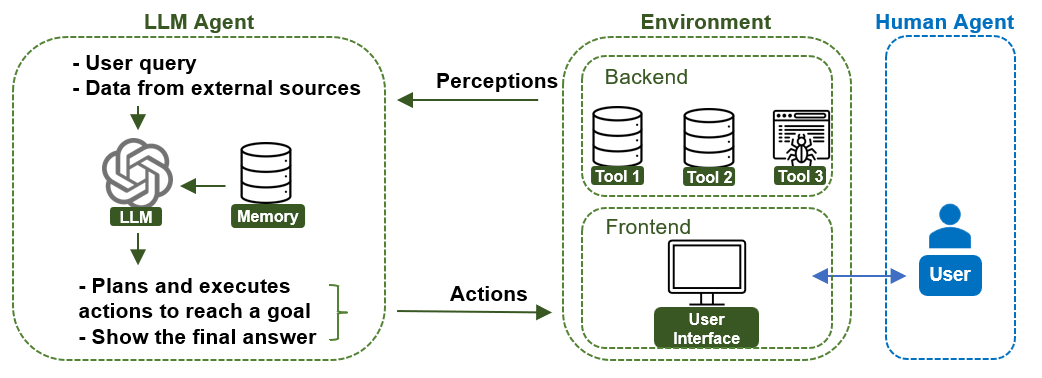
\includegraphics[width=0.75\textwidth]{images/agent_environment_4.png}
                \caption{Schematic of the LLM-based agent interacting with an environment containing tools for task-specific operations, and the Human Agent interface for user interaction and feedback.}
                \label{fig:agent_environment}
            \end{figure}           
            
            Initially, a configuration of agents was implemented as described in Figure~\ref{fig:agent_config_1} using AutoGen Framework \citep{Wu2023} with an architecture that allows information retrieval and user interaction. This system consists of two agentic setups:

            \begin{figure}[h]
                \centering
                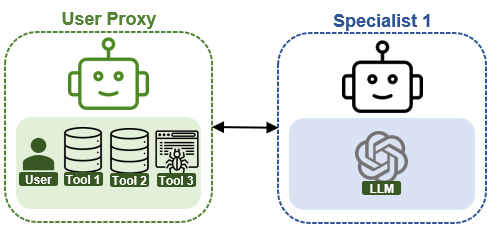
\includegraphics[width=.5\textwidth]{images/agent_config_1.png}
                \caption{Chat setup with one User Proxy \citep{Wu2023} and one Assistant.}
                \label{fig:agent_config_1}
            \end{figure}

            \begin{itemize}        
                        
                \item \textbf{User Proxy:} represents the interface with the user and with tools to access external databases. The modular nature of the tools allows the User Proxy to be customized and expanded based on the variety of data sources and the specific requirements of the application domain.

                \item \textbf{Agent:} powered by LLMs such as GPT-4 and GPT-3 (the specific model is configurable), is the analytical engine of the system. This agent interprets the queries received from the User Proxy and formulates responses.
                                    
            \end{itemize}

            
            For each question in the data set, the agent's decision-making process is executed as described in Figure~\ref{fig:diagrama_agente_1}, initially selecting the appropriate tool to respond to a query and, finally, compiling the retrieved information to provide a final answer.

            \begin{figure}[h]
                \centering
                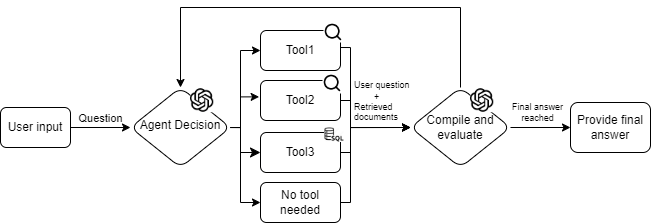
\includegraphics[width=0.75\textwidth]{images/agent_diagram_1.png}
                \caption{Decision process of the agent.}
                \label{fig:diagrama_agente_1}
            \end{figure}

        \subsection{Multi-Agent Architecture}

            The second artifact is a multi-agent system where responsibility is distributed among several specialized agents, coordinated by a Chat Manager, as shown in Figure~\ref{fig:agent_config_2}. This architecture is designed to handle queries by routing them to the agent best equipped for the task. As depicted in the decision process in Figure~\ref{fig:diagrama_agente_MultiAgente_2}, a \enquote{speaker selection} step determines the most suitable agent to act at each turn, promoting a more focused and contextualized approach to problem-solving.

            % (Your Figure agent\_config\_2 would be Figure 3.3 here)            
            \begin{figure}[h]
                \centering
                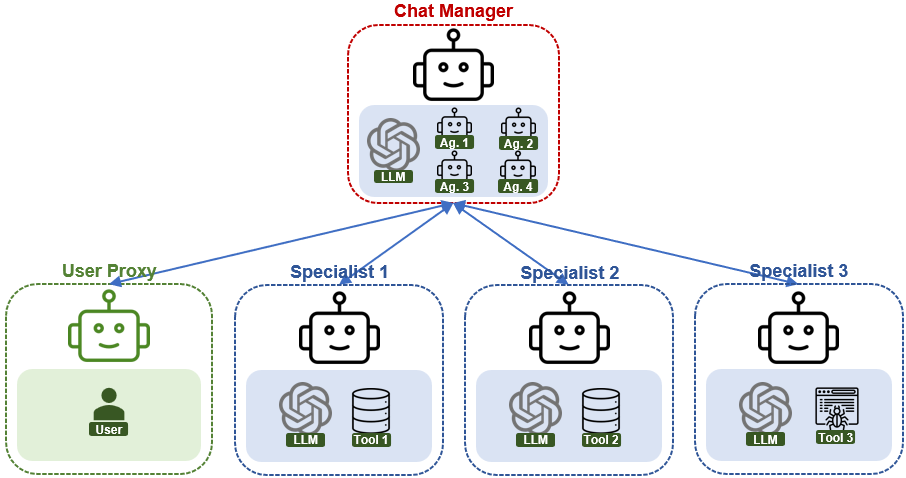
\includegraphics[width=.75\textwidth]{images/agent_config_2.png}
                \caption{Chat setup with one Chat Manager and a group of LLM agents.}
                \label{fig:agent_config_2}
            \end{figure}
            
            % (Your Figure diagrama\_agente\_MultiAgente\_2 would be Figure 3.4 here)
            \begin{figure}[h]
                \centering
                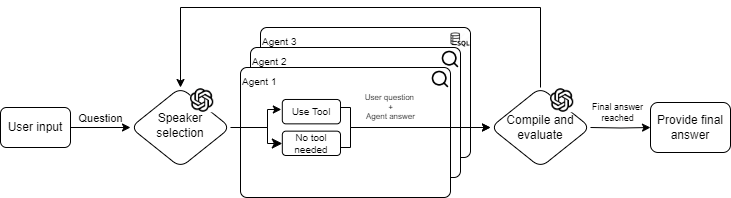
\includegraphics[width=1\textwidth]{images/agent_diagram_2.png}
                \caption{Multi-agent decision process.}
                \label{fig:diagrama_agente_MultiAgente_2}
            \end{figure}

                

        \subsection{Agent's Tools}
            
            In this experiment, three tools were considered in the decision-making process:

            \begin{itemize}            
                
                \item \textbf{Tool 1 - Learned Lessons Search:} a tool to search for learned lessons that may be relevant to the query. 
                \label{Tool1}
        
                \item \label{Tool2} \textbf{Tool 2 - Employee Search:} functionality that allows the search for information related to collaborators of an organization.
        
                \item \label{Tool3} \textbf{Tool 3 - NPT SQL Query:} Interface for executing SQL queries on a database of operational NPTs.    
                
            \end{itemize}

            There is also a pathway that allows the agent to provide a direct response, without the need to resort to other tools, presumably used when the LLM already possesses the necessary information.

    \section{Evaluation}

        The evaluation phase was designed to assess and compare the performance of the two proposed artifacts. This section details the methodology, the data set creation process, the metrics used, and the final results.

        \subsection{Evaluation Methodology}
        
            The evaluation was conducted by presenting a standardized set of questions to both the single-agent and multi-agent systems, using both GPT-3.5-turbo and GPT-4 models. The responses generated by each configuration were then collected and anonymized.

            A panel of three specialist engineers from the well construction department was tasked with analyzing the generated answers. Each specialist independently scored the responses based on the metrics described in Section~\ref{sec:evaluation_metrics}. The final score for each response was calculated by averaging the scores from the three experts, ensuring a robust and comprehensive assessment.
            
            \xexeo{Aqui seria bom fazer um BPMN do passo a passo do seu experimento, veja a figura 4.1 de\url{https://www.cos.ufrj.br/uploadfile/publicacao/3172.pdf}}
            \vitor{Feito}

            To provide a clear visual representation of the experimental workflow, a Business Process Model and Notation (BPMN) diagram is presented in Figure~\ref{fig:experimental_workflow}. This diagram illustrates the step-by-step process, from query submission to expert evaluation.

            \begin{figure}[h]
                \centering
                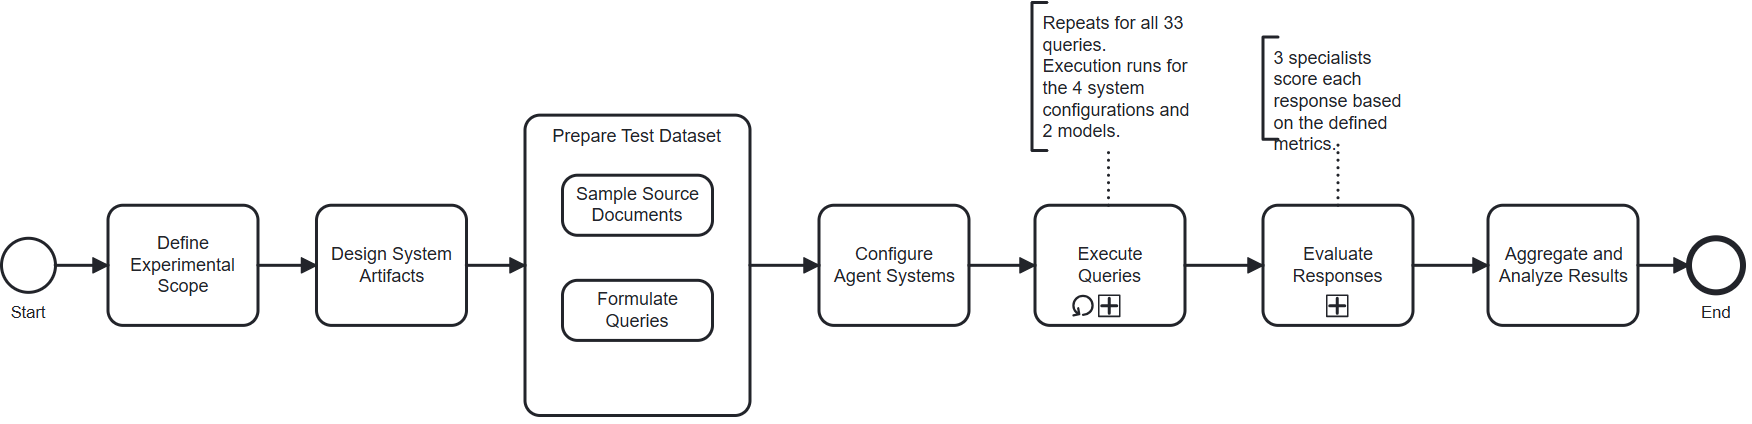
\includegraphics[width=\textwidth]{images/bpmn_experimento_1.png}
                \caption{Experimental workflow.}
                \label{fig:experimental_workflow}
            \end{figure}

            
        \subsection{Data Set Creation}

            A critical component of this evaluation is the test dataset. The dataset was meticulously created to reflect authentic information needs within the well construction domain. The process was as follows:

            \begin{description}
                \item[Source Selection] We identified three primary internal data sources: a database of Operational Learned Lessons, a structured database of Non-Productive Time (NPT) incidents, and a Collaborator Finder tool, as described in Section~\ref{sec:information-sources}.
                \item[Document Sampling] A random sample of documents and records was selected from each data source to ensure broad coverage of topics and scenarios.
                \item[Query Formulation] This process was performed by the author, leveraging domain expertise and collaboration with colleagues to ensure the questions were realistic, relevant, and challenging.
                \item[Dataset Composition] In total, a dataset of 33 unique queries was created. 
            \end{description}

            This approach to dataset creation, grounded in author experience and real-world documents, provides a valid basis for evaluating the artifacts. Table~\ref{table:question_examples} presents a sample of the queries formulated for the experiment.

            \xexeo{Coloca todas na tabela! E faz uma seção de criação de perguntas, ou subseção}
            \vitor{Feito}

            
            \begin{table}[h]
                \centering
                \scriptsize
                \sloppy
                \begin{tabular}{|p{.1\linewidth}|p{.9\linewidth}|}
                \hline
                \textbf{Task category} & \textbf{Question} \\   \hline
                \multirow{17}{*}{Q\&A} & How does the presence of silica in the composition of cement 
                paste affect its thermal stability at high temperatures? \\ \cline{2-2}
                & What are the main challenges and risks associated with through tubing plug and abandonment in highly deviated wells? \\ \cline{2-2}
                % & What can cause hydrate formation in the Tree Running Tool  connector during the HCR (High Collapse Resistance) hose flush  before connecting to the Wet Christmas Tree? \\ \cline{2-2}
                % & What can cause the Down Hole Safety Valve to remain open  due to hydrate formation in the control lines? \\ \cline{2-2}
                % & What can cause damage to thread protectors and sealing  areas of pin ends of pipes stored at the coating yard? \\ \cline{2-2}
                % & What can cause high drag and torque off-bottom during  the drilling of a well with high deviation? \\ \cline{2-2}
                % & What precautions should be taken when performing a top check  of the abandonment plug in wells with higher inclination? \\ \cline{2-2}
                % & What are the critical factors to consider when choosing a base  fluid for manufacturing a viscous support plug? \\ \cline{2-2}
                % & What are the best practices for managing drilling parameters  during cement cutting to avoid premature bit wear? \\ \cline{2-2}
                & Give me all the information about employee BFD1. \\ \cline{2-2}
                & Who are the employees of the POCOS/EP/SASD team? \\ \cline{2-2}
                & How many advisors do we have in the POCOS/SPO department? \\ \cline{2-2}
                & Who are the advisors in the departments belonging to the POCOS/EP department? \\ \cline{2-2}
                & What data sources do you have? \\ \cline{2-2}
                & What functions do you have? \\ \cline{2-2}
                & How does well inclination affect the effectiveness of cementing during through-tubing plugging? \\ \cline{2-2}
                & What can cause difficulty in locking the handling cap of the coiled tubing BOP? \\ \cline{2-2}
                & What can cause anomalous behavior of the AutoTrak with GunDrill during drilling? \\ \cline{2-2}
                & What can be done to optimize the assembly of COP/COI for parallel movement of the JRC/THRT? \\ \cline{2-2}
                & What strategies can be adopted to improve the quality of cementing in highly inclined wells during through-tubing plugging? \\ \cline{2-2}
                & What are the alternatives to accelerate the curing time of cement slurry without compromising its integrity in high-temperature conditions? \\ \cline{2-2}
                & What are the risks associated with the improper substitution of cement with silica for pure cement in surface casing cementations in high-temperature wells? \\ \cline{2-2}
                & What was the strategy adopted to allow the passage of eccentric and/or large-diameter elements through the BOP quickly and without wedging the string with these elements inside the BOP? \\ \cline{2-2}
                \hline                
                \multirow{15}{*}{Text-to-SQL} & What was the longest-lasting NPT on rig number 05? \\ \cline{2-2}
                & How many NPTs occurred on rig number 06 during August 2023? \\ \cline{2-2}
                & What were the 5 most common abnormalities across all rigs? \\ \cline{2-2}
                & What were the abnormalities that occurred on all rigs during the week of September 14th to 20th, 2023? \\ \cline{2-2}
                & Which rigs had the most lost time in 2023? Give me a table with the rigs and the sum of hours. \\ \cline{2-2}
                & Which rigs had the most lost time in the first half of 2023? \\ \cline{2-2}
                & What were the latest abnormalities that occurred on the SS-70 rig? \\ \cline{2-2}
                % & What was the longest-lasting abnormality on the SS-70 rig? \\ \cline{2-2}
                & What was the peak of abnormality occurrences on the NS-52 rig? \\ \cline{2-2}
                & What was the total lost time in hours for abnormalities whose description mentions the term "Coiled Tubing"? \\ \cline{2-2}
                & What was the total lost time in hours on the NS-38 rig in 2023? \\ \cline{2-2}
                & What was the total time lost due to equipment failure on the NS-38 rig in 2023? \\ \cline{2-2}
                % & How many abnormalities occurred on the NS-31 rig during August 2023? \\ \cline{2-2}
                & How many abnormalities occurred on the NS-31 rig during July 2023? \\ \cline{2-2}
                & How many hours of lost time were caused by human error on the NS-47 rig in 2023? \\ \cline{2-2}
                & How many hours of lost time occurred on the MS-20 rig during June 2024? \\ \cline{2-2}
                & How many hours of lost time occurred on the NS-35 rig in 2024? \\
                \hline
                \end{tabular}
                \fussy
                \caption{Queries used in first cycle. }
                \label{table:question_examples}
            \end{table}

        \subsection{Evaluation Metrics} \label{sec:evaluation_metrics}

            To ensure a comprehensive assessment, the expert panel evaluated the artifacts' responses using the following metrics, which are based on the definitions presented in Section~\ref{sec:evaluation-review}:

            \begin{itemize}

                \item \textbf{Truthfulness}: A 1-5 Likert scale score measuring the factual accuracy of the response and the extent of any divergence from the ground truth. A higher score indicates a more factually correct answer with no hallucinations.

                \item \textbf{Performance}: A 1-5 Likert scale score assessing the overall quality of the response, including its linguistic coherence, logical structure, relevance, and conciseness.

                \item \textbf{LLM Cost}: A quantitative metric representing the financial cost in US dollars (USD) to generate a response for a given query using the OpenAI API. This reflects the computational expense and efficiency of each configuration. While other costs exist (development, infrastructure, maintenance), the API cost is a primary operational expenditure that scales directly with usage and is therefore a key metric for evaluating the economic viability of the artifacts, as established in our DSR framework.
            
            \end{itemize}

            To illustrate the application of the first two metrics, an example of an expert evaluation is provided in Table~\ref{tab:tabela_inputs_example}. The table shows the responses of different models to the query: "How does the presence of silica in the composition of cement paste affect its thermal stability at high temperatures?". It details the scores for Truthfulness and Performance, along with the specialists' comments that justify the ratings.

            \xexeo{Por que essa pergunta? Isso é um exemplo? Como o multi agente entrou aqui se ainda não falou de multi agente? Melhor deixar para mais tarde ou mostrar só para single-agent?} 
            \vitor{Refatorado pra deixar claro q esse eh um exemplo e inserido após a explicação das arquiteturas.}
            % This 
            \xexeorem[comprehensive]{OLHA UMA PALAVRA INÚTIL TÍPICA DE LLM} 
            % comparison allows for an 
            \xexeorem[in-depth]{Outra} 
            % assessment of the models' capabilities in generating accurate and relevant responses to technical questions.
            \vitor{Essa parte com palavras típicas de llm foi escrita no artigo, início do ano passado, quando essas expressões ainda não eram indesejáveis kkkk estou retirando tudo. Se ainda tiver passado algo, me avise pfv.}


        \begin{landscape}
            \begin{table}[h]
            \small
            \centering
            \caption{Query example with inputs, outputs, and human expert evaluations.}
            \label{tab:tabela_inputs_example}
            \begin{tabular}{| m{3cm} | m{1.5cm} | m{1.5cm} |>{\scriptsize}m{9cm} | m{1.3cm} | m{1.2cm} |>{\scriptsize}m{4cm} |}                    
            \toprule
            % \textbf{Input query} & \textbf{Model} & \textbf{Setup} & \textbf{Final output} & \textbf{Truthfulness} & \textbf{Performance} & \textbf{Specialist \ Comments} \\
            Input query & Model & Setup & Final output & Truth. \newline fulness & Perfor- \newline mance & Specialist \ Comments \\
            \midrule
            How does the presence of silica in the composition of cement paste affect its thermal stability at high temperatures? & GPT-3.5-turbo & Single-Agent & The presence of silica in the composition of cement paste can affect its thermal stability at high temperatures due to some characteristics of silica. Silica is an inorganic material that has a stable crystalline structure at high temperatures. When exposed to high temperatures, the silica present in the cement paste can undergo structural transformations, resulting in changes in the properties of the paste.

            One of the main changes that can occur is the thermal expansion of the cement paste due to the formation of unstable silica compounds. This thermal expansion can lead to cracks and fissures in the structure, compromising the material's integrity and stability.

            Moreover, the presence of silica in the composition of cement paste can affect the material's thermal resistance. Silica has low thermal conductivity, which can lead to a reduced ability of the cement to withstand high temperatures. This can result in a decrease in the material's strength and, consequently, a reduction in its thermal stability.

            In summary, the presence of silica (...) & 4 & 5 & Created a section that is irrelevant to the question: "Moreover, the presence of silica in the composition of cement paste can affect the material's thermal resistance. (...)" \\
            \cline{3-7}
            &  & Multi-Agent & The presence of silica in the composition of cement paste has a positive effect on thermal stability at high temperatures. Silica is added to cement to mitigate the retrogression of cement strength when exposed to temperatures above 230°F (110°C). Deep wells or those with a high geothermal gradient may require the use of silica cement to ensure the thermal stability of the paste. The use of silica cement is particularly important in surface casing cementing, where the temperature can exceed the critical limit. \ (...) & 2 & 2 & Retrieved an unrelated Lesson Learned on the subject (about plugs). \\ 
            \cline{2-7}
            & GPT-4 & Single-Agent & The presence of silica in the composition of cement paste increases thermal stability, especially at high temperatures. Silica is used to transform the cement into a refractory material, capable of withstanding extreme conditions. 
            
            The cement (...).

            However, (...). & 3 & 4 & Although it is true, the item on the side is not relevant to the question: "However, it is important to note that (...)." \\
            \cline{3-7}
            &  & Multi-Agent & Silica is added to cement at a ratio of 35\% by weight of cement to mitigate the retrogression (loss of compressive strength) of the cement in the well when subjected to temperatures above 230ºF (110ºC). \ (...) & 5 & 4 & Cited an unrelated (but true) Lesson Learned about plugs, Lesson Learned LA7005. \\
            \hline
            \end{tabular}
            \end{table}
        \end{landscape}
            

        % \subsection{Results and Discussion}

            % (This section would contain the complete text from your original "Results" and "Discussion" sections. The content is good, but it logically belongs here as the final part of the DSR evaluation phase. You can simply move that text here, ensuring it flows from the description of the metrics.)


        \subsection{Results} % NEW SUBSECTION for your results
            % The results table and the sections analyzing each metric go here.
            % The original \subsection{Truthfulness}, \subsection{Performance},
            % and \subsection{LLM Cost} become \subsubsections.

            % The third metric, LLM Cost
            \xexeo{Isso aqui é uma pergunta de pesquisa tem que entrar de alguma maneira na definição do DSR, lembrando que as avaliações do DSR podem ser mais de uma}
            \vitor{Feito. Movido p/ definição do DSR}
            % , is
            \xexeo{Não é represents, já que é o custo mesmo, acho que  corresponds to, ou mesmo só is }
            \vitor{Feito} 
            % the financial cost associated with using OpenAI's API for the language models in each configuration. This metric is measured in US dollars and reflects the computational resources required for each task.
            \xexeo{Tem que falar alguma coisa que não é o único custo, e quais são os outros e porque esse é importante, isso pode estar descrito no modelo DSR, antes}
            \vitor{Feito}
            \xexeo{Esse parágrafo tipicamente aparece na revisão}


            This section provides an analysis of the data collected during the first experimental cycle. The aggregated results are presented in Table~\ref{tab:tabela_resultados}, followed by a discussion of each evaluation metric established in our DSR framework: Truthfulness, Performance, and LLM Cost.

            \begin{table}[h]
                \small % Reduce the font size
                \centering % Center the table on the page
                \caption{Results on Q\&A and Text-to-SQL tasks, including standard deviation (Std). The best metrics are highlighted with \textbf{\underline{bold and underline}}. The second best are highlighted with \textbf{bold}.}
                \label{tab:tabela_resultados}
                \begin{tabular}{|>{\raggedright\arraybackslash}p{2.0cm}|>{\centering\arraybackslash}p{0.85cm}|>{\centering\arraybackslash}p{0.95cm}|>{\centering\arraybackslash}p{0.8cm}|>{\centering\arraybackslash}p{0.8cm}|>{\centering\arraybackslash}p{0.8cm}|>{\centering\arraybackslash}p{0.85cm}|>{\centering\arraybackslash}p{0.95cm}|>{\centering\arraybackslash}p{0.8cm}|>{\centering\arraybackslash}p{0.8cm}|>{\centering\arraybackslash}p{0.8cm}|}
                \hline
                \rowcolor{gray!20}
                \textbf{Task}           & \multicolumn{5}{c|}{\textbf{Single-Agent}}           & \multicolumn{5}{c|}{\textbf{Multi-Agent}} \\ % Merging cells and adding heading
                \textbf{Model}          & \textbf{LLM Cost} & \textbf{Truth.} & \textbf{Std} & \textbf{Perf.} & \textbf{Std} & \textbf{LLM Cost} & \textbf{Truth.} & \textbf{Std} & \textbf{Perf.} & \textbf{Std} \\ \hline
                \cellcolor{gray!20} Q\&A & & & & & & & & & &\\
                GPT-3.5-turbo            & 0.005             & 2.94              & 1.48 & 3.94          & 1.09 & 0.02              & 4.09              & 1.22 & 3.82 & 0.98 \\
                GPT-4                   & 0.12              & \textbf{3.88}     & 1.41 & \textbf{4.06} & 1.30 & 0.45              & \underline{\textbf{4.57}} & 0.79 & \underline{\textbf{4.43}} & 0.79 \\
                \cellcolor{gray!20} Text-to-SQL & & & & & & & & & &\\
                GPT-3.5-turbo            & 0.009             & 4.13              & 1.41 & 4.44          & 1.03 & 0.02              & \textbf{4.29}     & 1.20 & \textbf{4.29} & 1.33 \\
                GPT-4                   & 0.10 & \underline{\textbf{4.56}} & 0.96 & \underline{\textbf{4.63}} & 0.81 & 0.51      & 3.20              & 1.99 & 3.70 & 1.89 \\ \hline
                \end{tabular}
            \end{table}

            The comparative analysis between single and multi-agent setups for RAG, using GPT-3.5-turbo and GPT-4 models, revealed insights regarding the metrics of truthfulness, performance, and costs of the language model.


            \subsubsection{Truthfulness} 

                In assessing the truthfulness metric, significant differences are noted between the single and multi-agent settings in both Q\&A and Text-to-SQL tasks. The results are illustrated in Figures \ref{fig:truthfulness_QA} and \ref{fig:truthfulness_text2sql}.
                For Q\&A tasks, GPT-4 in a multi-agent configuration significantly exceeded the performance of the single-agent with a truthfulness score of 4.57 compared to 3.88. The GPT-3.5-turbo model showed distinct results between the two configurations, with the multi-agent surpassing the single-agent with scores of 4.09 and 2.94, respectively.
                In terms of Text-to-SQL queries, a different outcome was observed. GPT-4 single-agent achieved a score of 4.56, while the same model in the multi-agent configuration obtained 3.20, highlighting a limitation for the multi-agent in this task. Conversely, the GPT-3.5-turbo maintained a more balanced performance between configurations, scoring 4.29 for multi-agent and 4.13 for single-agent.
                
                \begin{figure}[h]
                    \centering
                    \begin{minipage}{.48\textwidth}
                        \centering                
                        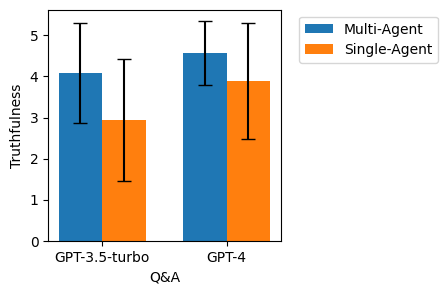
\includegraphics[width=1\linewidth]{images/truthfulness_QA.png}
                        \caption{Truthfulness and standard deviation in Q\&A tasks by LLM model and agent configuration.}
                        \label{fig:truthfulness_QA}
                    \end{minipage}%
                    \hspace{0.2cm}
                    \begin{minipage}{.48\textwidth}
                        \centering
                        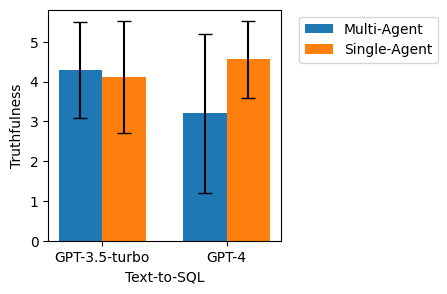
\includegraphics[width=1\linewidth]{images/truthfulness_text2sql.png}
                        \caption{Truthfulness and standard deviation in Text-to-SQL tasks by LLM model and agent configuration.}
                        \label{fig:truthfulness_text2sql}
                    \end{minipage}
                \end{figure}

                
            \subsubsection{Performance}        

                The evaluation of LLM performance \citep{Li2023} in the tasks of Q\&A and Text-to-SQL reveals trends which are similar to the truthfulness results. 
                % As shown in Figures \ref{fig:performance_QA} and \ref{fig:performance_text2sql} and summarized in \ref{tab:tabela_resultados}, the text performance in single and multi-agent setups was compared using the GPT-3.5-turbo and GPT-4 models.        
                For Q\&A tasks, the multi-agent setup shows a performance boost compared to the single-agent setup. In particular, the multi-agent GPT-4 achieves a performance score of 4.43, which is higher than the single-agent GPT-4 score of 4.06. This pattern is consistent with the GPT-3.5-turbo, where the multi-agent system also surpasses the single-agent system, scoring 3.82 and 3.94, respectively. These findings emphasize the effectiveness of the multi-agent approach in handling technical user queries.
                        
                \begin{figure}[h]
                    \centering
                    \begin{minipage}{.48\textwidth}
                        \centering                
                        % \framebox{
                            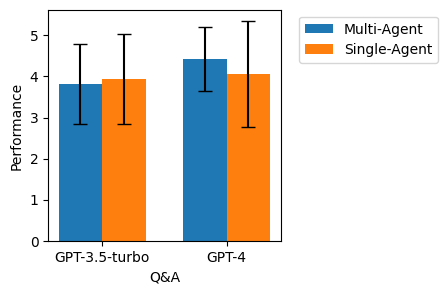
\includegraphics[width=1\linewidth]{images/performance_QA.png}
                        % }
                        \caption{Performance and standard deviation in Q\&A tasks by LLM model and agent configuration.}
                        \label{fig:performance_QA}
                    \end{minipage}
                    \hspace{0.2cm}
                    \begin{minipage}{.48\textwidth}
                        \centering
                        % \framebox{
                        % 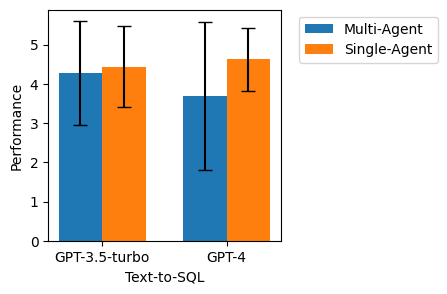
\includegraphics[width=1\linewidth]{images/performance_text2sql.png}
                        % }
                        \caption{Performance and standard deviation in Text-to-SQL tasks by LLM model and agent configuration.}
                        \label{fig:performance_text2sql}
                    \end{minipage}%
                \end{figure}


            \subsubsection{LLM Cost} 
                Language model services are typically composed by a values per token. For instance, GPT-4 model costs US\$30.00 (input) and US\$60.00 (output) per 1 million tokens received and sent, respectively.        
                The single-agent architecture demonstrated substantially lower costs for both Q\&A and Text-to-SQL tasks compared to the multi-agent setup as shown in Figure~\ref{fig:truthfulness_vs_cost_vs_config_model}. For instance, the average cost of the GPT-4 model \citep{OpenAI2023} for a Q\&A task was \$0.12 per processed question for the single-agent, while the multi-agent recorded an average cost of \$0.45. This trend of higher costs for the multi-agent architecture was also maintained for Text-to-SQL tasks, with an average cost of \$0.51 for the multi-agent architecture in contrast to \$0.10 for the single agent.
                The higher token count and cost for multi-agent setting is due to the inclusion of intermediate calls, for example, when the "Agent Selector" needs to decide which agent to pass the turn to. All the message history is passed to the LLM at this stage, substantially increasing the number of tokens submitted and response time.


                \begin{figure}[h]
                    \centering              
                    % \framebox{
                        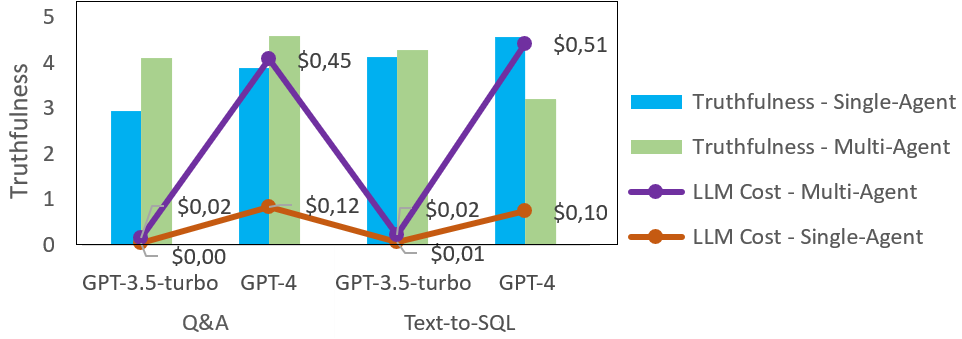
\includegraphics[width=0.75\textwidth]{images/truthfulness_vs_cost_vs_config_model.png}
                    % }
                    \caption{Average LLM costs and Truthfulness per completed task according to setup and model.}
                    \label{fig:truthfulness_vs_cost_vs_config_model}
                \end{figure}
                
                

        \subsection{Discussion} % NEW SUBSECTION for your discussion
            % The original \section{Discussion} and all its content go here.
            % The original \subsections become \subsubsections.

            
            The comparison between single and multi-agent systems revealed significant differences in terms of performance and cost:
            
            \subsubsection{General Performance.}     
                The results indicate that for Q\&A tasks in the context of O\&G, truthfulness measure was 28\% higher with the multi-agent architecture compared to single. 
                However, for Text-to-SQL tasks, this trend was inverted, where the single-agent scored 15\% higher.

                These findings suggest that for Q\&A tasks, the multi-agent setup may be more advantageous in terms of providing truthful information, particularly when utilizing the more advanced GPT-4 model. 
                Conversely, in Text-to-SQL tasks, the GPT-4 model in a single-agent configuration proved more effective. 
                This might imply that the added complexity of managing multiple agents in some tasks does not necessarily lead to improved performance in responses, underscoring the importance of carefully selecting the agent configuration based on the task type and specific features of the language model used.
                    
            \subsubsection{Cost-Performance Analysis.}
                While the multi-agent system shows higher truthfulness in Q\&A tasks, it is crucial to consider the associated costs. 
                To provide a clearer comparison, let us consider the score/cost ratios. For Q\&A tasks using GPT-4, the single-agent configuration yields a ratio of 32.33 truthfulness points per dollar, compared to 10.16 for the multi-agent setup. This indicates that while the multi-agent system shows a 17.8\% improvement in truthfulness, it comes at a 275\% increase in cost.
                
                % Based on our analysis, we recommend using a multi-agent system for Q\&A tasks when the budget allows for it and accuracy is a critical factor. 
                % However, decision-makers should consider setting a cost-performance threshold to guide the choice of system configuration, ensuring that the benefits justify the expenses involved.
                \xexeo{TEm que deduzir a necessidade de fazer um experimento antes levando essas coisas em consideração}
                \vitor{Feito abaixo.}

                This trade-off highlights an important implication for any organization considering the adoption of these technologies. The optimal architecture is not universal; it is highly dependent on specific task requirements and budget constraints. 
                This reality underscores the necessity of conducting a preliminary, cost-performance evaluation. Rather than simply selecting a model, decision-makers must first perform a targeted analysis to establish a cost-benefit threshold. 
                Our work not only provides initial data for the O\&G domain but also demonstrates a foundational methodology for this evaluation process, which ultimately motivated the more rigorous and quantitative approach of our second experimental cycle.


            \subsubsection{Model Performance Variations.}
                Interestingly, our results show that GPT-3.5-turbo outperforms GPT-4 in certain tasks, particularly in the Text-to-SQL multi-agent configuration, despite GPT-4's larger size and more extensive training. 
                This unexpected performance could be attributed to several factors. 
                First, GPT-3.5-turbo may have undergone more specific fine-tuning for structured query tasks, allowing it to excel in Text-to-SQL scenarios. 
                Additionally, GPT-3.5-turbo's training data might be more recent or more relevant to the specific domain of our study. 
                Another possibility is that the smaller model size of GPT-3.5-turbo allows for faster processing and more efficient handling of the multi-agent setup, resulting in better performance in some contexts.

                However, it is important to note that GPT-4, when used in a multi-agent setup, demonstrated more consistent truthfulness and performance, as evidenced by its reduced standard deviation in results. 
                This consistency can be particularly advantageous in applications where reliability and accuracy are critical. 
                Multi-agent systems have the advantage of maintaining separate contexts for different aspects of a task \citep{Langchain2025blogmultiagent}. 
                \xexeo{Você pode suportar essa afirmação com uma citação?}
                \vitor{Feito.}
                This compartmentalization can lead to better handling of complex, multi-faceted queries, as each agent can focus on its specific context without being overwhelmed by irrelevant information. However, this advantage may be offset in tasks like Text-to-SQL, where maintaining a unified context of the database schema and query structure is crucial, possibly explaining the better performance of single-agent setups in this task.
                Furthermore, the multi-agent architecture inherently involves multiple stages of information processing, which can serve as natural filtering mechanisms.
                As information passes from one agent to another, irrelevant or low-quality data may be naturally filtered out, leading to more refined and accurate final outputs. 
                This could explain the superior performance in filtering irrelevant information observed in multi-agent setups.
            
            
            \subsubsection{Economic Efficiency.} 
            
                The multi-agent architecture incurs significantly higher costs compared to the single-agent system, primarily due to additional intermediate calls to the language model and multiple iterations between agents for action planning. 
                Also, the cost differences between using GPT-4 and GPT-3.5-turbo are substantial, with GPT-4 being 20 times more expensive (in early 2024).
                \xexeo{Dizer x vezes mais caro em julho de 2025}.
                \vitor{Feito}

                The average cost per query for each configuration is presented in Table \ref{tab:cost_per_query}. These figures highlight the direct cost implications of the chosen architecture and model.
                
                \begin{table}[h!]
                \centering
                \caption{Average LLM Cost Per Query (USD). Values from early 2024.}
                \label{tab:cost_per_query}
                \begin{tabular}{l r}
                \toprule
                \textbf{Configuration} & \textbf{Cost per Query} \\
                \midrule
                Single-Agent (GPT-3.5-Turbo) & \$0.0068 \\
                Single-Agent (GPT-4) & \$0.1095 \\
                Multi-Agent (GPT-3.5-Turbo) & \$0.0197 \\
                Multi-Agent (GPT-4) & \$0.4896 \\
                \bottomrule
                \end{tabular}
                \end{table}

                To illustrate the financial implications of adopting different models and architectures, we estimate the annual costs for a large company with 40,000 knowledge workers. Our calculations are based on an average of 5 queries per worker per day, over 250 working days per year.
                
                Under these assumptions, the total annual query volume is 50 million (40,000 workers $\times$ 5 queries/day $\times$ 250 days). For a single-agent configuration, this results in an annual cost of approximately \$337,843 for GPT-3.5 and \$5.47 million for GPT-4.
                
                In a multi-agent architecture, the costs increase substantially, escalating to approximately \$986,631 for GPT-3.5 and \$24.48 million for GPT-4. These estimates underscore the significant financial trade-offs when adopting a multi-agent system, which, while potentially offering performance benefits, comes with a considerable increase in LLM operational costs.

                While multi-agent systems and more advanced models like GPT-4 offer improvements in performance, the economic efficiency, as measured by truthfulness per dollar, may favor single-agent systems and less costly models like GPT-3.5-turbo, depending on the specific application and budget constraints.

                It is important to note that, as of July 2025, the landscape of LLMs has evolved substantially. The emergence of more efficient models, has led to a significant decrease in API's costs. This suggests that the financial trade-offs discussed previously may no longer be as pronounced, and that high-performance multi-agent systems could become economically viable much sooner than anticipated.

                \xexeo{In summary é o parágrafo típico das LLMs... Mas é isso mesmo. Porém tem que colocar um ponto: o custo dos modelos está caindo barbaramente com o aparecimento de novos modelos no topo de desempenho e novas tecnologias tem permitido alcançar resultados de ótima qualidade com máquinas muito menores, o que também derruba o custo. Pode até citar o exemplo do DeepSeek (buscando na literatura o desempenho x custo dele)}
                \vitor{Feito}
                
            
            \subsubsection{Challenges and Limitations}     
                During the evaluation of the agents, several challenges and limitations were identified.

                \textbf{\textit{Contextualization and Interpretation.}} 
                    In many cases, the single-agent solution had difficulty understanding the context of the question. For example, a question about cementing was interpreted in the context of the construction industry, a theme to which the language models were more exposed during the training phase. 
                    However, the multi-agent structure, with its well-defined roles, better understood the questions and showed superior performance in Q\&A tasks, corroborating the findings of \citep{Li2024}.
                
                \textbf{\textit{Filtering Irrelevant Information.}} 
                    The agent often receives irrelevant documents along with important ones in the prompt context, and it is up to the LLM to ignore these. 
                    For example, when asked about alternatives to accelerate the curing time of cement paste without compromising its integrity at high temperatures, the RAG system retrieved a document that included information about batch cementing to ensure homogeneity during manufacturing and pumping. 
                    While this information is true, it was not relevant to the specific question asked. 
                    In this aspect, the multi-agent solution performed better at discarding such irrelevant information, focusing more accurately on the task at hand. 
                    Other possible solutions include improving the accuracy of semantic search by adjusting a minimum threshold for similarity measures or through re-ranking techniques such as those proposed by \citep{Carraro2024} and \citep{Sun2023}.
                
                \textbf{\textit{Hallucination.}} 
                    During the evaluation of our system, we encountered instances where the agent produced hallucinated information instead of utilizing the appropriate tool to retrieve accurate data, as in \citep{Bilbao2023}. 
                    For example, when asked, "How many anomalies occurred on rig number 05 during August 2023?" the agent was expected to use the Text-to-SQL tool to query the database. 
                    However, it bypassed this tool and generated a fabricated response, stating that 5 anomalies occurred, along with detailed descriptions of fictional events. The correct answer, as retrieved from the database, was that 7 anomalies occurred. This hallucination likely resulted from the agent's reliance on its internal knowledge rather than external data retrieval. 

                    In terms of hallucination statistics, our analysis revealed that for Q\&A tasks, hallucinations occurred in 9.6\% of cases and 3.8\% for partially hallucinated. 
                    In contrast, Text-to-SQL tasks exhibited a lower hallucination rate, with only 3.6\% of responses containing hallucinated information and 96.4\% being accurate. 
                    These findings highlight the variation of susceptibility to hallucination in different types of tasks, highlighting the need for targeted strategies to mitigate this problem.
                
                \textbf{\textit{Industry Jargon:}}
                    Specifically analyzing the activity of drilling and completion of offshore wells, the main challenge is the inherently complex and technical nature of the data involved. 
                    There were instances of incorrect interpretation of information, likely due to the use of terms, expressions, and themes specific to well construction, to which the language model had little or no exposure during training phase. 
                    A possible solution is the implementation of specialized models, which has been pointed out in gray literature as a trend for the coming years \citep{Shah2024, Meena2023, Ghosh2023}.
                
                \textbf{\textit{Tools vs. Performance:}} 
                    It was identified during the experiments that agents with a high amount of tools showed a decline in overall performance. 
                    This can be attributed to the added context to the prompts. 
                    As the context length increases, the model's ability to accurately interpret and respond diminishes.
                    This is a limitation of current language models, where longer contexts can lead to a dilution of relevant information and increased difficulty in maintaining coherence and accuracy. 
                    This conclusion is currently qualitative, as these metrics were not addressed in this experiment.

                
                \textbf{\textit{Queries Involving Proper Names:}}
                    In queries involving people's names, it was not possible to retrieve relevant documents using semantic search. 
                    For example, when asked to identify the employee associated with a specific key and list knowledge items they registered in the system, the LLM incorrectly attributed such documents to the wrong author
                    \xexeo{O RAG ou a LLM usando o RAG, não ficou claro}
                    \vitor{Corrigido}
                    . 
                    This highlights the difficulty in accurately retrieving information based on proper names, which can be complicated by variations in accentuation, abbreviation, and formatting.
                    \xexeo{tem evidências disso em outros artigos?}
                    \vitor{não encontrei}
                    A potential solution to be explored is the use of Self-Query Retriever \citep{LangchainSelfQuery2023}, implementing a hybrid search with metadata filters (including proper names) and semantic retrieval of the rest of the query. 
                    It is also suggested, in these cases, to use the \citep{Levenshtein1966} distance to handle possible variations in the spelling of names. 
                    This approach could improve the accuracy of retrieving documents related to specific individuals, ensuring that the correct information is associated with the right person.
                    
            
            % \subsubsection{Practical Implications}
            \subsubsection{Practical Implications.} 

                The findings from our study have significant practical implications for the O\&G sector, and potentially for other industries characterized by complex and technical data environments:
                    
                \begin{itemize}
                
                    \item \textbf{Enhanced Decision-Making Support:}
                        Our results indicate that multi-agent systems provide a 28\% higher truthfulness measure in Q\&A tasks. This can be particularly beneficial for decision-making in well engineering, where accurate and truthful information is critical.
                        Implementing multi-agent systems in decision-making processes can lead to more reliable and informed decisions, thereby reducing the risk of errors and enhancing operational safety and efficiency.
                    
                    \item \textbf{Balancing Performance and Economic Efficiency:}
                        While multi-agent systems offer superior performance in terms of truthfulness, they come with a cost that is 3.7 times higher on average compared to single-agent systems.
                        This highlights the importance of a strategic approach in selecting agent configurations based on specific tasks and budget constraints. 
                        % For instance, single-agent systems might be more cost-effective for Text-to-SQL tasks where they have shown to perform 15\% better. 
                        A detailed cost-benefit analysis reveals that for Q\&A tasks using GPT-4, the single-agent configuration yields a ratio of 32.33 truthfulness points per dollar, compared to 10.16 for the multi-agent setup. While the multi-agent system shows a 17.8\% improvement in truthfulness, this comes at a 275\% increase in cost. The efficiency varies significantly by task type; in Text-to-SQL tasks, the GPT-4 single-agent outperforms the multi-agent by 42.5\% in truthfulness while costing 80.4\% less. 
                        % These quantitative insights emphasize the need for careful consideration of task requirements and budget constraints when choosing between single and multi-agent configurations.
                        
                    \item \textbf{Reflection and Critic Agents:}
                        A promising approach to enhance the performance of these agents is the use of reflection \citep{Shinn2023}, a method where agents verbally reflect on task feedback signals and maintain this reflective text in an episodic memory buffer to improve decision-making in subsequent trials. Critic agents are a way to implement reflection in a multi-agent setup. This type of agent is challenging to apply in Q\&A tasks over private technical data, as commercial LLMs (OpenAI, Google Bard, and others) have not been deeply trained in the domain and struggle to provide relevant and precise critiques, reinforcing the trend toward increased use of domain-specific models \citep{Shah2024, Meena2023, Ghosh2023}.                
                        
                    \item \textbf{Task-Specific Agent Configuration:}
                        The study highlights that the complexity of managing multiple agents does not always lead to better performance. In some cases, a single-agent setup might be more effective.
                        This insight can guide the development and deployment of AI systems, ensuring that the configuration of agents is tailored to the specific requirements of the task, thereby optimizing both performance and cost.           
                        
                    \item \textbf{Potential for Broader Application:}
                        The insights gained from this study are not limited to the O\&G sector but can be applied to other industries with similar technical complexities, such as aerospace, pharmaceuticals, and renewable energy.
                        By adopting multi-agent systems in these industries, organizations can improve decision-making, knowledge management, and operational efficiency, driving innovation and competitiveness.             
                    
                \end{itemize}
                        
                    
            \subsubsection{Future Directions.} 

                This work indicates possible pathways for enhancing RAG architectures in O\&G sector. 
                
                \begin{itemize}
                
                    \item \textbf{Enhancement of IR Semantic Techniques:}
                        There is a critical need to develop more sophisticated semantic search technologies. Future efforts should focus on enhancing the precision of information retrieval by filtering out irrelevant content more effectively. This will ensure that agents can provide more accurate and contextually appropriate responses, crucial for technical domains such as O\&G.
                        
                    \item \textbf{Development of Domain-Specific Models:}
                        Specialized models tailored specifically to the O\&G and other domains, such as biomedical engineering \citep{Pal2024}, could significantly improve the handling of specific jargon and complex technical data, while reducing LLM costs \citep{Arefeen2024}. Future research should aim to develop and train these models to better understand and interpret the unique language and data types found in O\&G, enhancing the overall accuracy of agent responses.
                        
                    \item \textbf{Optimization of Tool Use in Agent Performance:}
                        The relationship between the quantity of tools available to an agent and its performance needs further exploration. Future studies should quantify the impact of tool availability on agent efficacy and efficiency, aiming to optimize tool use without overwhelming the agent or diluting performance quality.
                        
                    \item \textbf{Integration of Advanced Name Recognition Techniques:}
                        Queries involving proper names pose a significant challenge in semantic search. Integrating advanced retrieval techniques, such as Self-Query Retrievers \citep{LangchainSelfQuery2023} and \citep{Levenshtein1966} distance algorithms, could improve the handling of these queries. Future research should focus on enhancing name recognition capabilities to ensure that agents can accurately retrieve and utilize correct information, especially in scenarios where precision is paramount.
                        
                    \item \textbf{Extension to Other Complex Domains:}
                        The potential applications of multi-agent systems are not limited to the O\&G sector. Future research should explore the adaptation and implementation of these systems in other complex and technical domains, such as aerospace, pharmaceuticals, and renewable energy. Investigating how these systems can support decision-making in these areas will provide valuable insights into their versatility and adaptability.
                        
                    \item \textbf{Hybrid Model Experimentation:}
                        Combining the strengths of single and multi-agent systems could yield significant benefits. Future directions should include experimenting with hybrid models that integrate the robustness and depth of multi-agent interactions with the simplicity and efficiency of single-agent systems. This hybrid approach could potentially offer a balanced solution, maximizing performance while managing costs and complexity.
                        

                \end{itemize}
                
                By pursuing these directions, future research can significantly advance the development of multi-agent systems, not only enhancing their application in the O\&G sector but also expanding their utility across various technologically intensive activities.
                    